 \documentclass[conf]{new-aiaa}
%\documentclass[journal]{new-aiaa} for journal papers
\usepackage{preamble}
\usepackage{setspace}
\usepackage{amssymb}
\usepackage[utf8]{inputenc}
\usepackage{float}

\usepackage{graphicx}
\usepackage{amsmath}
\usepackage[version=4]{mhchem}
\usepackage{siunitx}
\usepackage{longtable,tabularx}
\usepackage{amsmath}

\begin{document}

\begin{titlepage}
    \begin{center}
        \vspace*{1cm}
        {\LARGE \textbf{Design Readiness Report} \\
        \vspace{0.5cm}
        \textbf{Team Toucan}} \\
        \vspace{0.5cm}
        {\normalsize
        \textbf{by} \\
        \vspace{0.5cm}
        \textbf{Joshua Clements, Chris Endres, Jack Johnson,\\ Mateusz Korzen, Kacper Piechnik and Nicole Zaworski} \\
        \vspace{0.5cm}
        {\large\textbf{AE443 Senior Design II}}\\
        \vspace{0.5cm}
        \textbf{February 13th, 2020}} \\
        \vspace{2.5cm}
        {\large University of Illinois at Urbana-Champaign \\ Department of Aerospace Engineering} \\ 
        {\Large
        $\bullet$\\
        \vspace{2.5cm}
        $\bullet$\\
        \vspace{2.5cm}
        $\bullet$\\
        \vspace{1.75cm}}
        {\normalsize
        \textbf{Faculty Advisor:} Dr. Jason Merret}\\
        \textcolor{red}{Include A/C drawings or team logo}
    \end{center}
\end{titlepage}

\newpage

\pagenumbering{roman}
\section*{Group Member Assignments Sheet (JJ)}
\begin{center}
    \begin{tabular}{ |p{3cm}||p{3cm}|p{3cm}|p{1.5cm}|p{3cm}| }\toprule
        %  \multicolumn{5}{c}{Team Roster} \\\midrule
         \textbf{Name} & \textbf{Primary Role(s)} & \textbf{Secondary Role(s)} & \textbf{AIAA ID} & \textbf{Signature} \\\hline
         Chris Endres & Mass Properties; \newline Structures & Landing Gear & 1082820 & \\
         Jack Johnson & Team Lead & Avionics & 761905 & \\ 
         Joshua Clements & Aerodynamics; \newline Stability \& Control & Interior Design & 761967 & \\ 
         Kacper Piechnik & Systems & Acoustics & 1108702 & \\ 
         Mateusz Korzen & Loads \& Dynamics; \newline Performance & ASM & 981691 & \\ 
         Nicole Zaworski & Propulsion & Certification; Cost & 1108732 & \\\bottomrule 
    \end{tabular}
\end{center}

\newpage
\tableofcontents

\newpage

\section*{Nomenclature (\textit{JC})}
\hspace{-0.5in}\textbf{Coefficients}
{\renewcommand\arraystretch{1.0}
\noindent\begin{longtable*}{@{}l @{\quad=\quad} l@{}}
    b & Wing Span \\
    c & Chord length \\
    $C_D$ & Wing Drag Coefficient \\
    % $C_d$ & Airfoil Drag Coefficient \\
    % $C_{D,i}$ & Induced Drag Coefficient \\ %will this later apply to the whole plane?
    % $C_f$ & Skin Friction Coefficient \\
    $C_L$ & Wing Lift Coefficient \\ %will this later apply to the whole plane?
    % $C_l$ & Airfoil Lift Coefficient \\
    % e & Oswald Efficiency Factor \\
    % FF & Form Factor Term for parasitic drag calculation \\
    % g & Gravity (Earth = 9.81 $\frac{m}{s^2}$ \\
    $h_p$ & Pressure Altitude \\
    % Isp & Specific Impulse \\
    % K & Drag due to lift factor \\
    % L/D & Lift to Drag ratio \\
    % LE & Leading Edge \\
    M & Mach Number \\
    % m & Total aircraft mass \\
    % MAC & Mean aerodynamic chord \\
    % $M_{cr}$ & Critical Mach number \\
    % $M_{dd}$ & Drag Divergent Mach number \\
    % n & Load factor \\
    % Q & Interference factor for parasitic drag calculation \\
    % $q_{\infty}$ & Dynamic pressure \\
    % Re & Reynolds Number \\
    % S & LE Suction \\
    % $\mathcal{S}$ & Wing Area \\
    SFC & Specific fuel consumption \\
    % T/W & Thrust-to-weight ratio \\
    % t & Airfoil thickness \\
    % t/c & Airfoil thickness-to-chord length ratio \\
    % TE & Trailing Edge \\
    % TO & Take-off \\
    % $V_{NE}$ & Never Exceed Speed \\
    % $V_{1}$ & TO Decision Speed \\
    % $V_2$ & TO Safety Speed \\
    $W_e$ & Empty Weight\\
    $W_f$ & Fuel weight \\
    % $W_o$ & TO Gross Weight \\
    % W/S & Wing Loading \\
\end{longtable*}}
\hspace{-0.5in}\textbf{Greek Symbols}
{\renewcommand\arraystretch{1.0}
\noindent\begin{longtable*}{@{}l @{\quad=\quad} l@{}}
    $\alpha$ & Angle of Attack \\
    % $\beta$ & Prandtl-Glauert Compressibility correction \\
    % $\delta_f$ & Flap Deflection \\
    % $\Lambda$ & Sweep Angle \\
    % $\epsilon$ & Unit Strain \\
    % $\gamma$ & Shearing Strain \\
    % $\Gamma$ & Wing Dihedral Angle \\
    % $\eta$ & Efficiency \\
    $\lambda$ & Wing Taper Ratio ($C_{tip} / C_{root}$) \\
    % $\mu$ & Viscosity \\
    % $\rho$ & Air Density \\
    % $\sigma$ & Air density ratio ($=\rho/\rho_o$) \\
    % $\tau$ & Unit Shear Stress \\
\end{longtable*}}
\hspace{-0.5in}\textbf{Abbreviations and Acronyms}
{\renewcommand\arraystretch{1.0}
\noindent\begin{longtable*}{@{}l @{\quad=\quad} l@{}}
    A/C & Aircraft \\
    AIAA & American Institute of Aeronautics and Astronautics \\
    AR & Aspect Ratio \\
    % AEI & All Engines Inoperative \\
    % APU & Auxiliary Power Unit \\
    % BFL & Balanced Field Length \\
    % BL & Boundary Layer \\
    % BPR & Turbofan engine bypass ratio \\
    % CAD & Computer Aided Design \\
    % CAS & Calibrated Airspeed \\
    % CER & Cost Estimated Relationship \\
    CFD & Computational Fluid Dynamics \\
    CFR & Code of Federal Regulations \\
    CG & Center of Gravity \\
    ConOps & Concept of Operations \\
    % CTOL & Conventional Take-off and Landing \\
    % DARPA & Defense Advanced Research Projects Agency \\
    % DoD & Department of Defense \\
    % EAS & Equivalent Airspeed \\
    FAA & Federal Aviation Administration \\
    FEA & Finite Element Analysis \\
    FAR & Federal Aviation Regulations (certification Spces) \\
    % FAR & Federal Acquisition Regulations \\
    % FBW & Fly By Wire \\
    % FOD & Foreign Object Damage \\
    ft & foot \\
    % GA & General Aviation \\
    % GPS & Global Positioning System \\
    % IAS & Indicated Airspeed \\
    % ICAO & International Civil Aviation Organization \\
    IFR & Instrument Flight Rules \\
    % ILS & Instrument Landing System \\
    % IPPD & Integrated Product and Process Development \\
    % IR & Infrared \\
    % IOS & International Standards Organization \\
    % JATO & Jet-Assisted Take off \\
    % KISS & KEEP IT SIMPLE, STUPID! (Ed Heinemmann) \\
    % LCC & Life-cycle cost \\
    % LOX & Liquid Oxygen \\
    % L\&P & Leakage and Protuberances \\
    % MDO & Multidisciplinary Design Optimization \\
    % MSL & Mean Sea Level \\
    MTOW & Maximum Take-off Weight \\
    % MZFW & Maximum Zero Fuel Weight \\
    % NASA & National Aeronautics and Space Administration \\
    % NAV & Navigation \\
    nm & nautical mile \\
    % NS & Navier-Stokes (high-end CFD) \\
    % OEM & Original Equipment Manufacturer \\
    % OEI & One Engine Inoperative \\
    % OML & Outer Mold Lines \\
    % RCS & Radar Cross Section \\
    % RCS & Reaction Control System \\
    % RFI & Request for Information \\
    RFP & Request for Proposals \\
    % RFQ & Request for Quotations \\
    % RPM & Revolutions per Minute \\
    % S\&C & Stability and Control \\
    % SL & Sea Level \\
    % SOP & Standard Operating Procedure \\
    % STOL & Short Take-off and Landing \\
    % TAS & True Airspeed \\
    % TVC & Thrust Vector Control \\
    % UAV & Unmanned Aerial Vehicle \\
    VFR & Visual Flight Rules \\
    % VTOL & Vertical Take-off and Landing \\
    % ZFW & Zero Fuel Weight\\
\end{longtable*}}


% \section*{List of Figures (Optional)}
% \section*{List of Tables (Optional)}

\newpage \setcounter{section}{0}
\doublespacing

\section{Executive Summary (\textit{JJ})}
The following design report represents the basis for a new aircraft developed by Team Toucan at the University of Illinois at Urbana-Champaign in response to AIAA's Request for Proposal\cite{RFP} addressing the industry need for a high capacity, short to medium haul widebody capable of mitigating the increased traffic and congestion found at many modern airports.  While the design aircraft will be capable of carrying up to 400 passengers up to 3,500 nm, it has been engineered to bridge the gap between low capacity, short range regional jets and high capacity, long range twin jets currently on the market.  This report validates the possibility of addressing the prescribed requirements in a commercial aircraft.

Prominent driving design points of the Sam Mark I include takeoff and landing distances under 9,000 ft, maximum range of 3,500 nm, capacity of 400 passengers and their respective luggage, 10 person crew (two pilots, eight flight attendants), starting cruise altitude of 37,000 ft, adherence to FAA 14 CFR Part 25 regulations and fundamental desire to maximize customer value through minimizing fuel consumption as well as other operating costs.  Cabin pressure will not exceed 8,000 ft, and five ft$^3$ of luggage space will be available per customer, increasing passenger comfort.  The proposed aircraft will be service ready by 2029 and has been designed as a twin engine, twin aisle widebody with a traditional tail.  Most notably, the entire wing including its sub-structure will be designed and manufactured utilizing modern composites to minimize structural weight while not sacrificing performance or longevity.  Other value-added design points include leading and trailing edge high lift devices, VFR and IFR flight with autopilot, and de-icing capability for flight in less than ideal weather conditions.

To date, preliminary sizing of the aircraft is nearing completion.  Important current parameters to define the aircraft include a cruise speed of Mach 0.9, MTOW weight of 550,000 lb, of which 75,000 lb are fuel, AR of nine, wing span of 212 ft, and mean aerodynamic chord of 328 in. The seed and fundamental based estimations in this report are fluid, and moving forward Team Toucan will be performing in-depth analysis of all major components to fully optimize the design to the driving design points.  Leading edge slats and trailing edge, 2-panel Fowler-type flaps will be designed and integrated into the wing structure to efficiently generate lift under critical conditions such as take-off and landing.  Final design will follow a detailed FEA and CFD analysis of the aircraft's aerodynamic surfaces and structure in order to ensure flight worthiness and will accompany a thorough approximation of assembly cost, timeline, and life cycle maintenance costs.  Additionally, a component wise weight build up of corrected values for hybrid construction will supplement an in-depth stability and control analysis.  Considerable effort will be put into meeting or exceeding applicable FAA 14 CFR Part 25 requirements for commercial aircraft, and final design will be completed within the next two months, with the vast majority complete in the next four weeks leaving adequate time for review, system integration check, and submission of a safe, value-driven aircraft design by May 14th, 2020.

\textcolor{red}{
\begin{itemize}
    \item Briefly discuss motivation for the aircraft, key requirements, and your design drivers. (JC \checkmark)
    \item Briefly  summarize the proposed aircraft, including key  characteristics (e.g. general configuration, \textbf{TOGW, primary dimensions), key performance metrics, key differentiators, and a cost summary.} (JC \checkmark)
    \item Include any requirements not met, struggling with, or have chosen to exceed. \textbf{(none?)}
    \item Discuss the near term milestones and provide a project timeline for the semester. 
    \item Maximum length: one page, single-spaced if necessary. (JC \checkmark)
\end{itemize}}

\pagenumbering{arabic} % MODIFYING PAGINATION FROM ROMAN TO ARABIC

\section{Introduction (\textit{JJ})}
The Sam Mark I has been developed to solve one of aviation's biggest challenges: congested airports in urban areas prone to significant delays.  As airlines continue to embrace the hub and spoke model, it becomes ever apparent modern aviation has ignored one of the biggest necessities in the market - a high capacity plane optimized to handle shorter routes while still retaining the capability of long-haul nonstop flight between the world's major destinations. A twin engine wide body, the Sam Mark I will be capable of comfortably carrying 400 passengers in a 50/350 2-class configuration with adequate range to fly transatlantic from the Eastern seaboard to European destinations.  Unlike many competitors, the Sam Mark I takes full advantage of contemporary composites and high-lift devices in order to feature a fully composite wing adjacent to traditional fuselage, resulting in a significant increase in performance and added value to the end user.  This value will only increase as populous economies across the world mature, resulting in an increased demand on commercial aviation and the existing infrastructure. % JJ
\textcolor{red}{
\begin{itemize}
    \item Discuss motivation, design objectives (e.g design drivers, key requirements), and a summary of key design characteristics and capabilities. 
    \item This section should identify your niche (i.e. who your target customers are), convince the reader to read the rest of the report, and provide context for the remaining discussion. 
    \item Discuss any unique attributes to your design philosophy. 
    \item Start pagination as: 1, 2, 3,... \checkmark
\end{itemize}}

\section{Concept of Operations (\textit{JC, MK})}
The design requirements that are followed in this report are given by AIAA Request for Proposal, which are outlined in Table \ref{uno}.

\begin{table}[h!] 
    \centering
    \caption{RFP Requirements}
    \begin{tabular}{ |c||c| }\toprule
    \textbf{Category} & \textbf{Requirement} \\\hline\hline
    Capacity & 410 (10 crew, 400 passengers) \\\hline
    Payload & 94,000 lb (200lb per person, 30lb per occupant) \\\hline
    Range & 3,500 nm \\\hline
    Takeoff Field Length & 9,000 ft with a 35 ft obstacle \\\hline
    Landing Field Length & 9,000 ft \\\hline
    Approach Speed & 145 kts at end of design mission\\\hline
    Pressure & 8,000 ft pressure altitude at maximum flight altitude \\\hline
    Certification & Flying qualities should meet CFR Part 25.\\\hline 

    \end{tabular}\label{uno}
\end{table}

\hl{If additional requirements are made by group, discuss here. Will also include figure of design mission once decided on, and discuss it.}


\textcolor{red}{
\begin{itemize}
    \item AIAA: A description of the design missions defined for the proposed concepts for use in
calculations of mission performance as per design objectives. This includes the
selection of cruise altitude(s) and cruise speed/cruise Mach supported by pertinent
trade analyses and discussion.
    \item Discuss requirements (including those from the RFP and any additional derived requirements), constraints, and the design mission.
    \begin{itemize}
        \item Include a table of requirements.
        \item Include a figure of the design mission with key mission segments labeled and details noted (e.g. cruise range and altitude).
    \end{itemize}
\end{itemize}}

\section{Sizing Analysis (\textit{KP})}
The initial sizing analysis was conducted by examining a variety of similar aircraft and making sure to satisfy all the requirements given by the AIAA RFP \cite{RFP}. Some of the analyzed aircraft included the Boeing 777-200, Boeing 787-100, Airbus A340-600, and the Lockheed L-1011-100, which all featured similar capacities and ranges.  Once compiled, the aircraft were assigned a quantitative rank from one to seven based on  capacity and range. Sorting by composite score, the Boeing 777-200 was chosen as the main seed aircraft due to its highest perceived similarity to a hypothetical plane developed for the RFP. Some key parameters derived from seed analysis and RFP mandates are presented in Table \ref{tab:req}; a list of all candidate aircraft considered in the sizing analysis are listed in Table \ref{tabmk1}, as the same subjects were used in the Section \ref{section: Configuration} trade study.

\begin{table}[h!] 
    \centering
    \caption{Key Parameters}
    \begin{tabular}{ |c||c| }\toprule
    \textbf{Parameter} & \textbf{Value} \\\hline\hline
    Payload & 94,000 lb  \\\hline
    Range & 3,500 nm \\\hline
    Takeoff Field Length with a 35 ft obstacle & 9,000 ft  \\\hline
    Landing Field Length & 9,000 ft \\\hline
    Cruise Speed & 487 kts\\\hline
    Cruise Altitude & 37,000 ft \\\hline
    Max Takeoff Weight & 550,000 lb\\\hline 
    L/D & 17.83\\\hline 
    $C_{L_{max}}$ & 1.65\\\hline 
    SFC & 0.65\\\hline 

    \end{tabular}\label{tab:req}
\end{table}

Parameters compiled from the similarity analysis were approximated by taking historic averages of those respective to the different analyzed aircraft. Preliminary cruise speed was obtained by assuming an average cruise Mach of 0.9, while initial cruise altitude was estimated by taking averages of similar aircraft. Many other sizing parameters, specifically the wing geometries, were calculated using equations from Raymer \cite{raymer}. The wing area, however, was calculated by taking a couple averages of seed aircraft as an initial value of 4,600 ft$^2$. This value was used to determine other wing related parameters, and was fine tuned as the sizing process went along. With all estimated parameters, an iterative process was used with a sizing spreadsheet to converge all sizing values for the initial Sam Mark I. This step was necessary due to the significant differences in range from all contemporary widebody, 300+ capacity commercial aircraft which could have been used as a seed.  The aircraft's weights were roughly calculated using a build up method, instead of taking the seed aircraft's weights, equations from Raymer \cite{raymer} and an initial assumption of 75,000 lb of fuel. A separate trade study was also conducted to address some key sizing parameters regarding the aircraft's fuselage to make sure that the Sam Mark I featured enough room for the designed seating arrangement. The trade study is demonstrated in Table \ref{tab:trade_params}.

\begin{table}[!h] 
    \centering
    \caption{Trade Study}
    \begin{tabular}{ |c||c||c| }\toprule
    \textbf{Aircraft} & \textbf{Fuselage Length [ft]} & \textbf{Max Takeoff Weight [lb]} \\\hline\hline
    Boeing 777-200 & 205.7 & 535,087  \\\hline
    Boeing 787-100 & 224.0 & 560,000  \\\hline
    Lockheed L-1011-100 & 177.8 & 466,079  \\\hline
    Airbus A340-600 & 228.2 & 390,307  \\\hline

    \end{tabular}\label{tab:trade_params}
\end{table}

\newpage

After analyzing multiple aircraft, a fuselage length of 210 ft was decided in order to hold more passengers than the Boeing 777-200, and to support a 3-4-3 economy seat arrangement. After utilizing a weight build up method, a max takeoff weight of 550,000 lb was calculated, which is about 15,000 lb heavier than the main seed aircraft. Once the weights were calculated, the total drag was able to be computed at desired takeoff conditions. This allowed for a computation of required takeoff thrust to be about 71,500 lbf. 


% \textcolor{red}{\begin{itemize}
%     \item AIAA: A description or graphical representation of the aircraft sizing based on the
% requirements and design objectives given. \hl{This should describe or represent the
% quantitative justification for the wing area and thrust of the aircraft that was selected.} 
%     \item Discuss the team’s similarity analysis and the rationale behind the aircraft selection. \checkmark JJ
%     \item Discuss what data was extracted from the similarity analysis. \checkmark JJ
%     \item Discuss a part by part build up and how it compares to the seed analysis \checkmark JJ
%     \item Discuss initial sizing and constraint analysis. 
%     \begin{itemize}
%         \item Include a table of key parameters used with justification for their values. \checkmark JJ
%         \item Include at least takeoff, landing, cruise, service ceiling, and \hl{loiter constraints.}
%     \end{itemize}
%     \item Include at least two trade studies that uses quantitative analysis to support design decisions made. \hl{I split into the sizing \& then fuse sizing as the "second" one}  Maybe tie into the trade study Mat outlined right below? I put a possible bridge in the first paragraph to it if you want to go that route. 
%     \item Include the aircraft allocated and derived requirements and their justifications: \hl{(I think he might want this for all of the planes we used? Open to interpretation)}
%     \begin{itemize}
%         \item $\frac{L}{D}$
%         \item $C_{L,max}$
%         \item SFC
%         \item Weights
%     \end{itemize}
% \end{itemize}}

\section{Configuration (\textit{MK})}
\textcolor{red}{
\begin{itemize}
    \item Discuss external configuration alternatives considered and design choices made.
    \item Discuss selected aircraft configuration design (i.e. distinctions between variants, major features, design characteristics/objectives).
    \item Include at least one trade study that uses quantitative or qualitative analysis to support design decisions made.
    \item Discuss the landing gear philosophy.
    \item 3-View drawing (VSP acceptable).
    \item Discuss future work
\end{itemize}}

Many configurations of aircraft were considered during initial design phase. First, a trade study was performed over similar aircraft that are either currently in service or have flown in the past. Table \ref{tabmk1} describes seven aircraft and some of their external configuration characteristics. 

\begin{table}[H]
    \centering
    \caption{Quantitative Trade Study of Similar Aircraft}
    \begin{tabular}{|m{3cm}|c|c|c|c|c|}
    \hline
    \label{tabmk1}
    \textbf{Aircraft} & \textbf{Tail Type} & \textbf{Wing Type} & \textbf{\# of Engines} & \textbf{2-class Seating} & \textbf{\# of Decks} \\
    \hline
    Boeing 777-200 & Conventional & Low & 2 & 375 & Single \\
    \hline
    Airbus 340-600 & Conventional & Low & 4 & 440 & Single \\
    \hline
    Boeing 787-10 & Conventional & Low & 2 & 330 & Single \\
    \hline
    McDonnell Douglas MD-11 & Conventional (w/ engine) & Low & 3 & 323 & Single \\
    \hline
    Lockheed 1011-100 & Conventional (w/ engine) & Low & 3 & 304 & Single \\
    \hline
    Boeing 747-400 & Conventional & Low & 4 & 496 & Double \\
    \hline
    Airbus 350-900 & Conventional & Low & 2 & 315 & Single \\
    \hline
    \end{tabular}
\end{table}

From the trade study, all seven of described aircraft featured a low-level wing along with a conventional tail. This is most likely due to the low-level wing providing space for a retractable landing gear along with simplicity of design. Thus, the has decided to go with a low-level wing.

The next external configuration decision was between a T-tail conventional tail. While the T-tail does reduce the risk of the tail stalling, it is much more difficult to design as the vertical tail has to support the entire weight of the horizontal tail. Alternatively, conventional tails are lighter and provide more simplicity in terms of design. Another benefit with conventional tails is that it offers more space to store fuel for the aircraft. As shown from the trade study, conventional tails are very widely used in commercial aircraft in today's market. Thus, the team has decided to use a conventional tail configuration. 

Furthermore, the number of engines on our aircraft along with the number of decks on the aircraft were to be decided. The team decided to go with a single-decker to provide simplicity in design as well reduced cost in manufacturing. Moreover, two engines were chosen for our aircraft, mainly for the reduced maintenance cost of more engines as well as a smaller fuel cost. The proven reliability of modern engines in trans-oceanic flights also played a role in deciding to have two engines. Figure ....... shows an OpenVSP model of the aircraft. 


\subsection{Seating Configuration}
The aircraft internal configuration is a two-class seating with business and economy seating accommodations.  Per AIAA RFP requirements, it is stipulated

\section{Propulsion (\textit{NZ})}



In order to create a basis for the engine choice, similar aircraft were chosen and examined. These aircraft, such as the Boeing 777-300, Airbus A330-300, Airbus A330-900, and Airbus A350 XWB, have a similar passenger capacity as the one required in the design competition, however have a much higher range capability. The primary drivers for the design of the propulsion system are the power requirement for the aircraft, as well as reliability. Since the aircraft will be used as a high capacity transport for short mission durations, it is vital that the engines can withstand a constant cycle of maximum take off thrust at a higher interval than tradition engines which experience longer flight durations. 

\subsection{Engine Comparisons}

The following engines, seen below, are used in similar aircraft with great success: Pratt \& Whitney PW4000, General Electric GE90-115B, Rolls-Royce Trent XWB, and Rolls-Royce Trent 7000.

\begin{table}[!h]
    \centering
        \caption{Comparison of Engines on Similar Aircraft}
    \begin{tabular}{|c||c|c|c|c|}\toprule
         & \textbf{PW4000} & \textbf{GE90-115B} & \textbf{RR Trent XWB} & \textbf{RR Trent 7000} \\\hline \hline
         \textbf{Aircraft} & Airbus A330-300 & Boeing 777-300 & Airbus A350 XWB & Airbus A330-900\\ \hline
         \textbf{Maximum Takeoff Thrust} & 52,000 - 62,000 lbs \cite{PW} & 110,000 lbs \cite{ge90} & 84,200 lbs \cite{xwb} & 71,110 lbs \cite{butterworth}\\ \hline
         \textbf{Dry Weight} & 12,900 lbs \cite{FAApw} & 19,316 lbs \cite{ge90} & 16,043 lbs \cite{xwb2} & 10,550 \cite{butterworth} \\ \hline
         \textbf{Cost per Unit} & - & \$ 27.5 million \cite{gecost} & - & \$ 11 million \cite{butterworth} \\ \hline
         \textbf{Bypass Ratio} & 4.9 \cite{PW} : 1 \cite{PW} & 9 \cite{safran} & 9.6 : 1 \cite{xwb} & 4.89 : 1 \cite{butterworth} \\ \hline
         \textbf{Fan Diameter [in]} & 94 \cite{PW} & 135 \cite{ge} & 118 \cite{xwb} &  97 \cite{butterworth}\\ \hline
         \textbf{Thrust to Weight} & 4.80-4.03 & 5.69 & 5.24 & 6.74 \\ \bottomrule
    \end{tabular}
    \label{tab:enginecomp}
\end{table}

While the aircraft are similar in capacity, the range on these aircraft is much higher than what is required for the Sam Mark I. As such, an assumption is made that the engines chosen for these aircraft may not be as reliable as necessary for the Sam Mark I, since the engine for the Sam Mark I will experience higher intervals of maximum thrust, leading to more fatigue to the engine. 

In order to validate our choice of a turbofan engine, which was also the type of engine of choice for the similar aircraft compared above, Figure ~\ref{PropSelection} was used along with the Mach speed the Sam Mark I will fly at cruise conditions, 0.9. This figure was used to quickly determine which propulsion systems are overpowered for the flight conditions that the aircraft will fly and rule out which propulsion systems would not be able to meet the flight conditions.

\begin{figure} [h!]
    \centering
    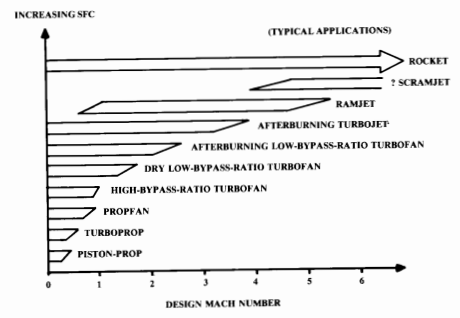
\includegraphics[width=0.8\textwidth]{Photos/PropSelection.PNG}
    \caption{Propuslion system speed limits. \cite{raymer}}
    \label{PropSelection}
\end{figure}

\newpage
With a Mach number of 0.9, both piston-prop and turboprop engines are not able to meet the speed requirement for cruise. The propfan propulsion system, while it may be able to handle a Mach number of 0.9, is not ideal as it is operating at the end of its limit. Scramjet and ramjet propulsion systems are over powered for the Sam Mark I system, leaving only three classes of turbofan engines and an afterburning turbojet engine. According to Raymer, the propulsion system should be one which the lowest on the chart for the specified Mach number, which for our case is the high-bypass-ratio turbofan \cite{raymer}. In addition, all of the engines listed in Table \ref{tab:enginecomp} are high-bypass-ratio turbofan propulsion systems as well, which gives confidence in the high-bypass-ratio turbofan engine being the propulsion system of choice for the Sam Mark I, barring any critical design concerns.


\subsection{Future Progress}

To solidify an engine choice, the sizing requirements and values that were generated by the team will be used to form a power requirement guideline for the propulsion system. This power requirement will be the primary driver for the choice of an engine as it will ensure that the engine chosen is not overpowered and that it will perform as necessary. Taking into account the need for the engine to be highly reliable as it may experience higher rates of fatigue due to the short mission, reliability will be the secondary driver for the propulsion system. The cost will be considered as well, however it will not be as prioritized as the goal is to design and choose as reliable of a system as possible.


%% Or...:
% \begin{wrapfigure}{r}{0.5\textwidth}
%     \centering
%     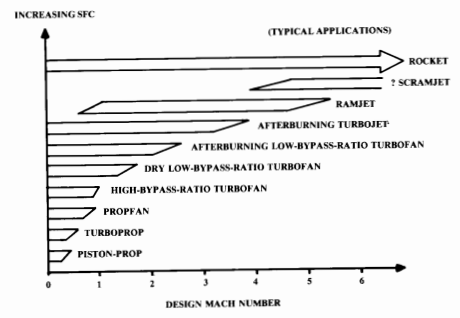
\includegraphics[width=0.5\textwidth]{Photos/PropSelection.PNG}
%     \caption{Caption}
%     \label{fig:my_label}
% \end{wrapfigure}

% \textcolor{red}{
% \begin{itemize}
%     \item Discuss overall propulsion system philosophy/design/selection.
%     \item Discuss future work.
%     \item AIAA: Propulsion system description and characterization including performance,
%     dimensions, and weights. The selection of the propulsion system(s), sizing, and
%     airframe integration must be supported by analysis, trade studies, and discussion
% \end{itemize}}

\newpage
\section{Aerodynamics (\textit{JC})}
\subsection{Airfoil Analysis}
The desired cruise conditions for the aircraft fall within transonic speed regime.  This provides favorable conditions for the sizing analysis but results in an increase in wave drag force.

\begin{wrapfigure}{r}{0.5\textwidth}
    \centering
    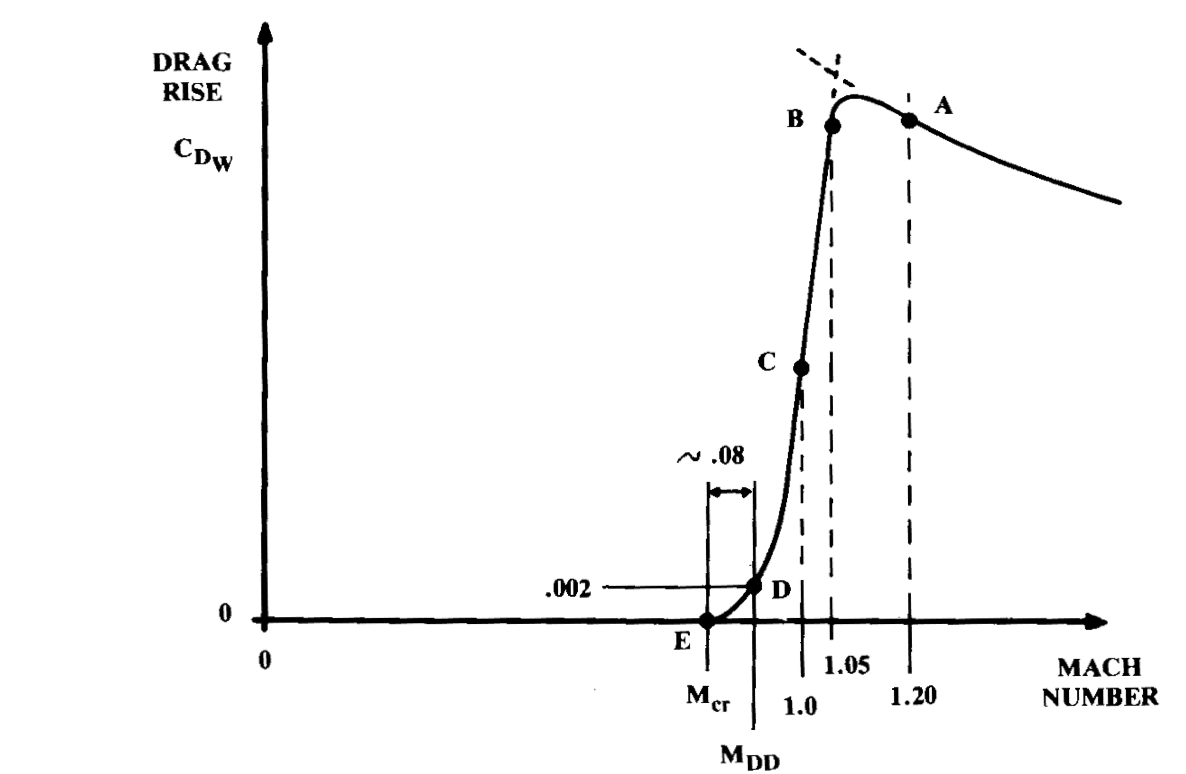
\includegraphics[width=0.5\textwidth]{Photos/wavedragduetotransonic.png}
    \caption{Wave Drag due to Transonic Airspeed\\{\small From Raymer Fig. 12.29\cite{raymer}}}
    \label{fig:transonic}
\end{wrapfigure}

As shown above in figure \ref{fig:transonic}, there is an increase in wave drag as the aircraft passes into the transonic regime.  Therefore, a selection of supercritical airfoils and wing sweep of no less than $30\degree$ is proposed in mitigation of the above trend.  To properly predict and quantify the wave drag for aerodynamic analysis on the airfoil and wing design, the \textit{Delta Method} and \textit{Method B} from Vargas\cite{vargas} shall be included in the part-by-part drag buildup.

\subsection{Wing Design}

\subsection{Drag Buildup}

\subsection{High-Lift Systems}

\subsection{Future Progress}


Will talk about supercritical airfoil analysis, run-through preliminary XFLR5 data, and general drag buildup. - Josh
\textcolor{red}{
\begin{itemize}
    \item Discuss wing design, including reasoning.
    \item Discuss high-lift system, including reasoning.
    \item Discuss drag buildup (tabulated) used to support sizing analysis.
    \item Discuss future work.
    \item AIAA: Important aerodynamic characteristics and aerodynamic performance for key mission
    segments and requirements (shared w/ aero)
\end{itemize}}

\section{Performance (\textit{MK})}
\subsection{Mandatory Performance (\textit{JJ, MK})}
The AIAA RFP \cite{RFP} requires this short range aircraft to have a maximum range of 3,500 nm while having the ability to carry a maximum capacity of 400 passengers in a dual class configuration. The aircraft must also have enough reserves to fly to an alternate airport 200 nm from the destination airport, hold for 30 minutes at the alternate airport, and contain 5\% contingency fuel, which is defined as 5\% of non-reserve block fuel. Furthermore, both takeoff and landing distances are restrained to 9,000 ft or less off asphalt or concrete runways including ISA + 15 degrees C. Finally, the maximum approach speed the aircraft can have is 145 KCAS at the end of the design mission. 

\subsection{Predicted Performance (\textit{MK})}
First-cut analysis was performed using an estimated empty weight as well as a fuel weight calculated by using a TSFC average of contemporary large turbofan engines, such as what would be found on an aircraft of this size.  This data was then input into a time-step integration spreadsheet to converge on a first design for a bounded range for cruise. For the duration of cruise, the aircraft will begin cruising at an altitude of FL370, where it will perform two step climbs of 3000 ft. each and end at a cruising altitude of FL430. Before and after cruise, the aircraft will follow the mission profile as stated in Section \ref{section: Conops} in Figure \ref{fig:missionprof}.

In the future, the flight envelope as well as fuel estimation of each segment in the mission profile will be performed. Additionally, the time-step integration of cruise will be refined and the time-step integration process will be implemented for the climb, descend, and loiter segments of the mission. Further analysis will performed on determining the drag of each mission segment as well as regulating that the design stays within the requirements set forth by the RFP. 

% \textcolor{red}{
% \begin{itemize}
%     \item Discuss performance analysis for takeoff and cruise supporting the sizing analysis.
%     \item Discuss future work.
%     \item AIAA: Aircraft performance summaries shall be documented and the aircraft flight envelope
%     shall be shown graphically
%     \item AIAA: Payload range chart(s)
%     \item AIAA: Important aerodynamic characteristics and aerodynamic performance for key mission
%     segments and requirements (shared w/ aero)
% \end{itemize}}

\section{Stability and Control (Optional/\textit{JC})}
A

\textcolor{red}{
\begin{itemize}
    \item Discuss any analysis supporting the sizing analysis.
    \item Discuss future work.
    \item AIAA: Summary of basic stability and control characteristics; this should include, but is not
    limited to static margin, pitch, roll and yaw derivatives.
\end{itemize}}

\section{Structures and Loads (CE)}
\subsection{Structures}
\subsubsection{Material Selection (\textit{CE})}
Modern-age aircraft exhibit many different structure layouts and material selection for each structure. The goal for the material selection is to meet the given requirements, as well as provide an aircraft which will have the best mechanical properties for the given flight missions. The different structure types are tabulated in Table \ref{tab:structure_material_table}.

\begin{table}[!h]
\centering
\caption{Structures Build-up Descriptions }
\label{tab:structure_material_table}
\begin{tabular}{ |p{2cm}||p{13cm}| }
\toprule
\multicolumn{1}{|c||}{\textbf{Build-up Type}} & \multicolumn{1}{c|}{\textbf{Description}}                                                                                                                       \\ \hline\hline
Metal                                       & Most or all parts of the primary and secondary structure are metallic, such as aluminum, steel, and titanium alloys                                             \\ \hline
Composite                                    & Most or all parts of the primary and secondary structure are composite, such as carbon fiber reinforced polymers (CFRP), fiber glass, or other composites \\ \hline
Hybrid                                       & Depending on the structure, the material of the structure is either metal or composite                                                                            \\ \bottomrule
\end{tabular}
\end{table}
% \begin{tabular}{ |p{3cm}||p{3cm}|p{3cm}|p{1.5cm}|p{3cm}| }

Metallic build-up is the more traditional method of designing aircraft structures, where most or all primary structures are composed of metal alloys. This method of construction is typically cost-effective and weight efficient for most structures, however, there are downsides such as damage tolerance and fatigue. A composite build-up requires high development costs, and relatively high manufacturing costs, but can offer incredible weight-savings compared to metal structure due to their high strength-to-weight ratio. In Fig. \ref{fig:strength_density}, the ultimate tensile strength versus the density of the material can be seen for many different categories of materials. Note that composites have a higher strength to weight ratio that most metal alloys. 

\begin{figure}[!h]
    \centering
    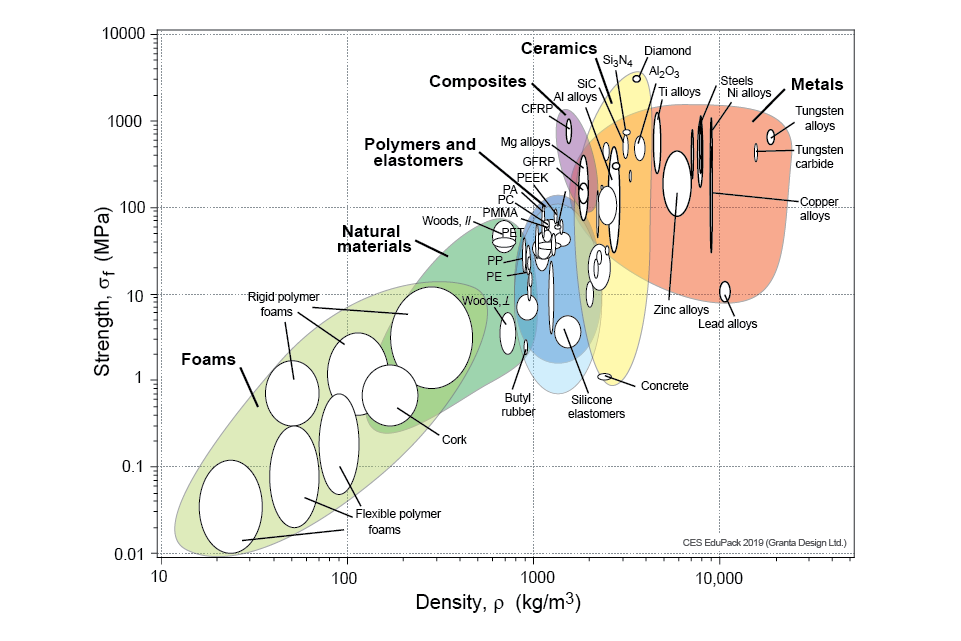
\includegraphics[width=\linewidth]{Photos/strength_density.png}
    \caption{Strength versus Density for Different Materials \cite{ashby}}
    \label{fig:strength_density}
\end{figure}

A hybrid build-up is a method where both metals and composites are used for different structures depending on key factors such as fatigue, damage tolerance, ultimate strength per density ratio, cost of manufacturing, assembly methods, and operational costs. Hybrid designs usually optimized costs and weight of the structure, which results in the wings and stabilizers to be a mainly composite build-up, and the fuselage and other secondary structures to be a metal build-up. Hybrid construction is a newer technology, and as the development of manufacturing of composites advances, this style of construction may become more prevalent in industry. A notable aircraft which uses a hybrid build would be the Boeing 777-X, in which the wings and stabilizers are composite and the fuselage is metallic. The reason the fuselage is metallic and not composite comes down to the difficulties in manufacturing a round and continuous composite structure, such as the fuselage and empennage sections. A notable aircraft which utilizes mainly composite construction is the Boeing 787, as seen in Figure \ref{fig:787 materials}.

\begin{figure}[!h]
    \centering
    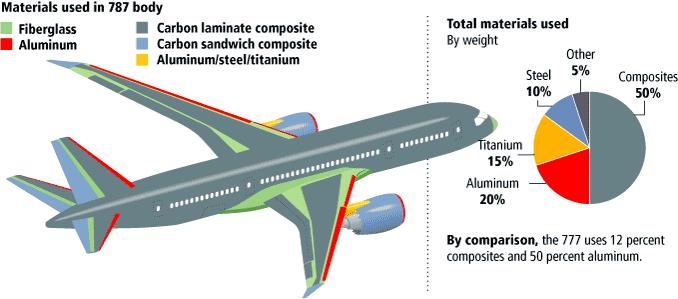
\includegraphics[width=\linewidth]{Photos/787 Materials.png}
    \caption{Material Composition of the B787 \cite{787_Mat}}
    \label{fig:787 materials}
\end{figure}

\FloatBarrier
In Table \ref{tab:pugh_structures}, the benefits and costs for each build-up construction method were weighed in a Pugh matrix given the requirements of cost reduction and the desired aspect ratio and wingspan.

\begin{table}[!h]
\centering
\caption{Pugh Matrix for Structures Material Selection}
\begin{tabular}{|p{3.5cm}||p{2cm}|p{2cm}|p{2cm}|p{2cm}| }
\toprule
\multicolumn{1}{|c||}{\textbf{Criteria}} & \multicolumn{1}{c|}{\textbf{Weight}} &  
\multicolumn{1}{c|}{\textbf{Metallic}} & \multicolumn{1}{c|}{\textbf{Composite}} & \multicolumn{1}{c|}{\textbf{Hybrid}} \\ \hline \hline 
Cost & 10 & 9 & 7 & 8 \\ \hline
Manufacturability & 8 & 8 & 5 & 7 \\  \hline
Strength to Weight & 8 & 7 & 8 & 9 \\  \hline
Fatigue Rating & 5 & 6 & 8 & 7 \\  \hline
Damage Tolerance & 5 & 7 & 6 & 7 \\  \hline
Corrosion Resistance & 4 & 4 & 9 & 8 \\  \hline
Environmental Impact & 3 & 8 & 4 & 6 \\  \hline \hline
 & \textbf{Total} & \textbf{315} & \textbf{292} & \textbf{328} \\
\bottomrule
\end{tabular}
\label{tab:pugh_structures}
\end{table}
\FloatBarrier

Given the Pugh matrix, a hybrid construction is most ideal for the given aircraft requirements. A low fidelity analysis of the structure can assume an isotropic material with the mechanical properties of an ideal composite layup to create a factor to apply to estimations of structure loading given by Raymer \cite{raymer}. A high fidelity analysis of the composite structure would require one of two methods: run FEA on an isotropic material with similar properties to an ideal composite layup, or run FEA with a specific composite build-up in a capable software such as ANSYS.

\subsubsection{Construction and Layout (\textit{CE})}
Given the hybrid construction method, the wings and stabilizers require a newer method of construction compared to the traditional metallic construction. Since composite layups are essentially an additive manufacturing technique, the stringers can be integrated into the upper and lower panels of the wings and stabilizers. This alone saves incredible costs and weight by eliminating the use of fasteners in high-load locations. The absence of fasteners increases the damage tolerance and fatigue rating of the structure as well.

Spars are the most important structure to the wings, and arguably the most important on the entire aircraft. These few parts make the entire aircraft fly, and in the process, see a lot of loading cycles over the life of the aircraft. In metal structures, loading cycles cause fatiguing, and then fatigue cracking, which degrades the structure. Traditionally, metallic structures use a 3-piece build-up for the spar: chord on the top and bottom, and a web connecting the two chords. This structure ends-up looking like a C-channel extrusion. The reason the spars are a 3-piece build-up comes down to crack growth and fatigue. A crack starts in the lower chord, but cannot grow through the entire spar since the chord is connected to the web by fasteners. There are a few aircraft that have used a one-piece, or monolithic, metallic spar, some being the Boeing 1-B and the Airbus 320 NEO. There is significant research in learning crack-growth patterns and predicting where cracks will start and grow; opening-up huge possibilities in reducing manufacturing costs by allowing optimized metallic spars to be utilized on low-cost aircraft.

\newpage
The spars are where composites differ greatly from traditional 3-piece spar construction. Since composite structures do not crack like metal structures when fatigued, a monolithic spar can be utilized. This spar construction reduces costs, but increases the weight due to a thicker layup compared to a simpler 3-piece construction. Due to the considerable cost savings, a monolithic composite spar may be the best option. Future work is needed to compare the different spar construction methods.

Ribs in the wings are traditionally multi-piece substructures comprised of machined aluminum parts. The benefit to using aluminum ribs in the wing comes from the fact that composites are difficult to utilize on very complex and dramatic geometry. Due to this fact, a metallic rib layout would minimize costs. In an effort to save more cost and manufacturing troubles, a monolithic rib structure, with the rib posts, chords, webs, and pads machined from a single billet of aluminum, can be investigated. Ribs in the stabilizers are typically not as complex as a rib in the wings due to the lower-loaded structure. In the stabilizers, composite ribs may be utilized for weight savings.

Since the fuselage is a metallic structure, a common layout of frames, stringers, and floor joists can be utilized. The floor joists may be a composite part, as the joists are not primary structure, and the connection method to the frames of the fuselage is by brackets and fasteners. Frames will be dispersed evenly along the length of the fuselage, with several frames being considered "floating", or not connected to the skin of the fuselage, and others being traditional frames. The floating frames are only mounted to the stringers, rather than the actual skin of the fuselage. Floating frames increase fatigue life, as fewer holes are introduced into the fuselage skin.

\subsubsection{Wing Attachment}
There are two primary methods of mating the wings and the fuselage: "bolt-on" or "drop-in". These methods are both commonly used in industry, as both offer different advantages and carry their own disadvantages. 

A "bolt-on" method essentially bolts the wings onto the fuselage through the wingbox, as the wingbox is integrated into the fuselage. Utilizing shear plates or tension bolts, each wing is attached to the fuselage using fasteners. This method is preferred by most aircraft manufactures, as manufacturing of the fuselage with an integral wingbox and two separate wings is easier to manage in most cases. Using fasteners to attach the wing to the fuselage from the outside poses a difficult engineering challenge which is to make sure load paths are correctly transferring load to the correct primary structures.

The "drop-in" method refers to dropping the fuselage into the space made by the wingbox and wing superstructure. In this method, the wings and wingbox are a singular structure, and the fuselage does not have an integral wingbox. Due to the wings and wingbox being connected before the mating to the fuselage, a more robust connection to the wingbox (internal connection of the spars to the wingbox, rather than fasteners) can be achieved. 

Given that the aircraft is a wide-body, large wingspan structure, a bolt-on method would be preferred, as the manufacturing and logistical challenges in a "drop-in" method are costly.

\subsubsection{Future Work for Structures (\textit{CE})}
Future work includes several key tasks. First item to tackle is the creation of the full CAD model of the aircraft. With the full model, FEA can be completed on the wing and/or fuselage structure. In the CAD model, the wing structure will have a higher detail than the fuselage sections, mainly due to the importance of the analysis of the wing. Second, simple hand calculations of the wing must be done in order to size the spars and stringers. Finally, structure sizing can be somewhat optimized via the higher fidelity FEA from the full CAD model.

\subsection{Loads (\textit{MK})}

One important aspect in the structural analysis of the aircraft is determining the limits in the performance of the aircraft. This is specifically done using a V-N diagram, as shown in Figure \ref{figVN}. This diagram incorporates parameters such as wing loading and performance velocities (maneuvering, cruise, and dive velocities) along with limit loading factors. Maximum positive and negative limit loading factors of 3.2 and -1.5 were chosen, respectively, according to the regulations set forth in FAA 14 CFR Part 25.337, Limit Maneuvering Load Factors. These limit loading factors also contain a safety factor of 1.5, as specified in FAA 14 CFR Part 25.303, Factor of Safety. Note that the velocities displayed in the diagram (Figure \ref{figVN}) is that the units are displayed as equivalent velocities (KEAS).

\begin{figure}[H]
    \centering
    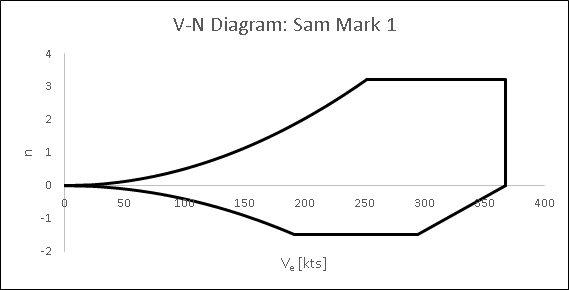
\includegraphics[width=\linewidth]{Photos/VN_Diagram_(2-11-20).png}
    \caption{VN Diagram of Limit Load Factors}
    \label{figVN}
\end{figure}

Future work includes derivation of a max dive speed and an updated V-N diagram with gust loads and changes due to sizing variations on the final aircraft. Additionally, a quantitative justification of a non-unique load safety factor remains.  

% \textcolor{red}{
% \begin{itemize}
%     \item Discuss any analysis supporting the sizing analysis.
%     \item Discuss future work.
%     \item AIAA: A V-n diagram for the aircraft with identification of necessary aircraft velocities and design load factors.
%     Required gust loads are specified in 14 Code of Federal Regulations (CFR) Part 25. (This may not come until later)
%     \item AIAA: Materials selection for main structural groups and general structural design, including layout of primary airframe structure as well as the strength capability of the structure
%     and how that compares to what is required at the ultimate load limits of the aircraft.
%     The maximum dive speed of the aircraft shall be specified. (this may not come until later)
% \end{itemize}}

\section{Mass Properties (CE)}
\subsection{Comparison Analysis}
\label{subsection: comparison}
Using the aircraft in Table \ref{tab:trade_params}, the fidelity of the mass estimation equations found in Roskam Part 2 \cite{roskam_2}, Roskam Part 5 \cite{roskam_5}, and Raymer \cite{raymer} can be quantified. By choosing the equations which closely fit the values seen in the real aircraft from the trade study rather than equations which may over or under estimate the mass, a higher fidelity prediction of the total mass of the aircraft can be created. At this time, little analysis has been done in terms of mass properties of the aircraft.

\subsection{Future Work}
Future work includes several tasks, such as creating a parametric spreadsheet using equations found in Roskam and Raymer and key parameters from the aircraft size to estimate the center of gravity location and the weight of the aircraft. This method would provide a low fidelity estimation, but by using the best equation for each section of the aircraft as described in \ref{subsection: comparison}, a higher fidelity solution can be reached. Another method of estimating the mass properties of the aircraft would be to create a high-detailed CAD model of the aircraft, where materials are assigned to each part of the structure with enough detail such that the weight, center of gravity, and moments of inertia can be estimated via the CAD software. 






% \textcolor{red}{
% \begin{itemize}
%     \item Discuss any analysis supporting the sizing analysis.
%     \begin{itemize}
%         \item Mass property methods chosen for different parts of the aircraft.
%         \item Estimate CG location.
%     \end{itemize}}
%     \item Discuss future work.
%     \item AIAA: Aircraft weight statement, aircraft center-of-gravity envelope reflecting payloads and fuel allocation. Establish a forward and aft center of gravity (CG) limits for safe flight. (may come later...con't on AIAA doc)
% \end{itemize}}

\section{Landing Gear (CE, JJ)}
The aircraft will feature three bogeys of retractable landing gear customary of that found on similar aircraft within the \hl{ref. trade study} of comparable aircraft.  Tentatively, the front assembly will be composed of two wheels, and the rears two symmetric sets of three wheels.  All bogeys will be hydraulically mounted to dampen the impact seen upon touchdown.  The three-bogey arrangement is traditionally seen due to both the stability of three on uneven surfaces as well as the weight distribution of the aircraft.  The front gear will also feature the main taxi light.  

@Chris: not sure if terminology is what you wish to use (e.g. bogey, etc)

Future work will consist of an analysis of the load and stress placed on the landing gear during taxi, takeoff, and, most importantly, landing.  Additional consideration will be taken to ensure the landing gear and its related hydraulic \hl{and pneaumatic/electrical?} systems stow within the contour of the fuselage as developed by aerodynamics.  Furthermore, brake sizing and fitment inside the wheel will be verified.  



% \textcolor{red}{
% \begin{itemize}
%     \item Discuss landing gear placement and design approach.
%     \item Discuss future work.
% \end{itemize}}

\section{Systems (Optional (\textit{KP}))}
The Sam Mark I includes every system that is compulsory in order to satisfy the given requirements meanwhile optimizing the aircraft's safety, and comfortability. The Aircraft's main systems are flight controls, deicing systems, engine control systems, environmental control systems, fuel systems, battery systems, along with an electrical and hydraulic system. These systems were chosen to provide the aircraft with the latest system technologies that are not present in older aircraft, and to provide safe flights. Due to the fact that the Sam Mark I is a large aircraft, each system has a redundancy factor built into it in case of a malfunction of any part. There are currently no schematics or demonstration figure in this report, but there will be in the final report. Other future work includes discussion of multiple types of the same system, and why the chose type is best suited for the Sam Mark I. 

\subsection{Flight Controls}


\section{Cost Analysis (Optional/\textit{NZ})}





% \textcolor{red}{
% \begin{itemize}
%     \item Discuss any analysis supporting the sizing analysis.
%     \item Discuss future work.
%     \item AIAA: Summary of cost estimate and a business case analysis. This assessment should
%     identify the cost groups and drivers, assumptions, and design choices aimed at the minimization of production costs. (con't on RFP)
%     \item AIAA: A lifecycle Carbon Dioxide (CO2) emission estimate. This estimate should include CO2
%     emissions from manufacturing the aircraft as well as CO2 emissions while in service. (could also go w/ prop)
% \end{itemize}}

\section{Conclusion (\textit{JJ})}
Utilizing widespread market comparison studies of eight contemporary aircraft closely fitting the RFP requirement range and/or capacity from different manufacturers, eras, and nations, the team was able to formulate an initial design fulfilling or exceeding the requirements for a 400 passenger, short to medium haul aircraft. Additionally, decisions have been made to utilize newfound technological advantages in composites and high-lift devices in order to optimize  an aircraft of this size for short haul (hundreds of nm) flights.  The first steps towards iteratively sizing and measuring the performance of this aircraft have been made, as has a foundation for strong justification of team decisions regarding the detailed design of the aircraft.

A considerable amount of work remains in regards to further optimization of the aircraft's subsystems, with special attention regarding the wing and structure in order to fulfil the team goal of designing the optimal high capacity, short range aircraft.  Additionally, substantial verification of FAA CFR requirements throughout all aspects of the aircraft remain.  Finally, significant strides will be made defining the aircraft's hydraulic, electrical, and environmental control systems, including adaptation of a state of the art avionics suite fulfilling the autopilot requirements set forth by AIAA.  By the conclusion of the final report, Toucan's Sam Mark I will have a build up analysis of each major system outlined in this report, as well as an estimation of production timelines and both initial and service-life maintenance cost.  Throughout this project, the team at Toucan has strode to develop a value-driven aircraft capable of exceeding client expectations while solving one of industry's toughest and omnipresent problems by applying a blend of new and proven technology and methodology to the design of Toucan Sam Mark I.  



% \textcolor{red}{
% \begin{itemize}
%     \item Summarize your motivation, design objectives, proposed design, key performance metrics, and key differentiators. 
%     \item Discuss problems encountered (e.g. requirements not met) and recommendations for future study (if any). 
%     \item Summarize future work. 
% \end{itemize}}

% \section{Appendix (Optional)}

% \section{AIAA Requirements}
% % \begin{table}[h!]
%     \centering
%     \caption{Numerical Requirements}
%     \begin{tabular}{|c|c|} \toprule
%         Range & 3,500 nmi \\\hline
%          & 
%     \end{tabular}
%     \label{tab:my_label}
% \end{table}

\bibliography{references.bib}

\end{document}
